\RequirePackage{fix-cm}
\documentclass[11pt,a4paper]{article}
\usepackage[spanish,es-nodecimaldot,es-noshorthands]{babel}
\usepackage[utf8]{inputenc}
\usepackage[margin=22mm]{geometry}
\usepackage{graphicx,booktabs,tabularx,array,caption,fancyhdr,hyperref}
\hypersetup{hidelinks,pdftitle={Figuras de la simulación exacta}}
\graphicspath{{figures/}}
\setlength{\parindent}{0pt}
\setlength{\parskip}{5pt}
\newcolumntype{Y}{>{\raggedright\arraybackslash}X}
\pagestyle{fancy}
\fancyhf{}
\fancyhead[L]{\small Optimización de Cobertura Territorial mediante Grafos}
\fancyhead[R]{\small Anexo visual}
\fancyfoot[C]{\thepage}
\renewcommand{\headrulewidth}{0.4pt}
\captionsetup{font=small,labelfont=bf}
\begin{document}

\begin{titlepage}
\centering
\vspace*{45mm}
{\Large Universidad Diego Portales\par}
\vspace{5mm}
{\large Proyecto de Grafos y Algoritmos\par}
\vspace{28mm}
{\LARGE\bfseries Figuras de la simulación\\con solución exacta\par}
\vspace{10mm}
{\large Anexo para explicar la construcción y resolución del modelo\par}
\vfill
{\large Octubre de 2026\par}
\end{titlepage}

\section{Datos de entrada y territorio}

La simulación utiliza localidades con población y un modelo digital de elevación (DEM). Las dos áreas mostradas son pilotos acotados: Biobío se procesa con ALOS PALSAR de 12,5 m y Metropolitana con Copernicus GLO-30 de 30 m. Los puntos representan las localidades incluidas; el relieve se utiliza en la evaluación de línea de vista.

\begin{figure}[h]
\centering
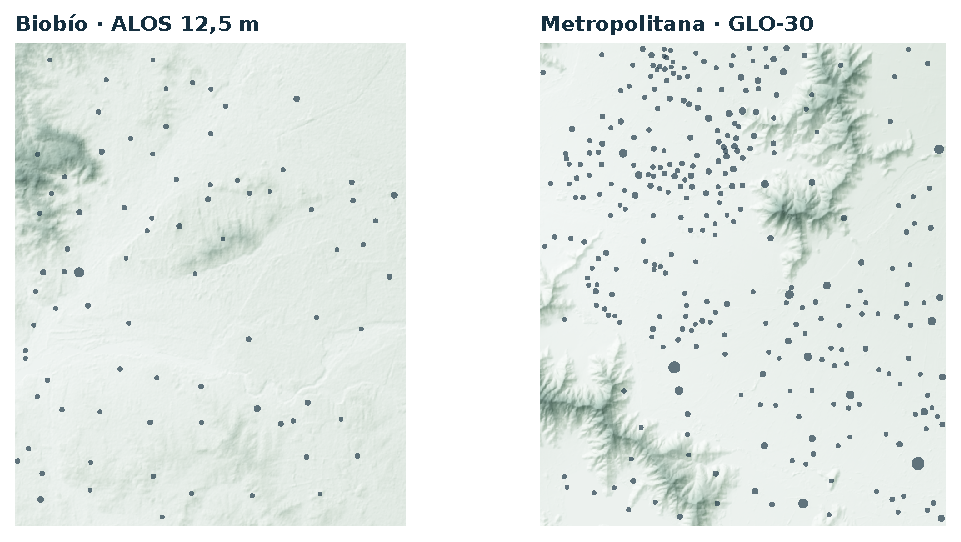
\includegraphics[width=.92\linewidth]{overview.pdf}
\caption{Territorio, relieve y localidades usadas en los dos pilotos de la solución exacta.}
\end{figure}

\clearpage
\section{Construcción de las aristas}

Una arista se incorpora al grafo sólo cuando la distancia entre candidato y localidad es admisible y el perfil del DEM no bloquea la línea de vista. La primera situación de la Figura~\ref{fig:los} genera una arista; la segunda queda fuera del grafo debido a una obstrucción del terreno.

\begin{figure}[h]
\centering
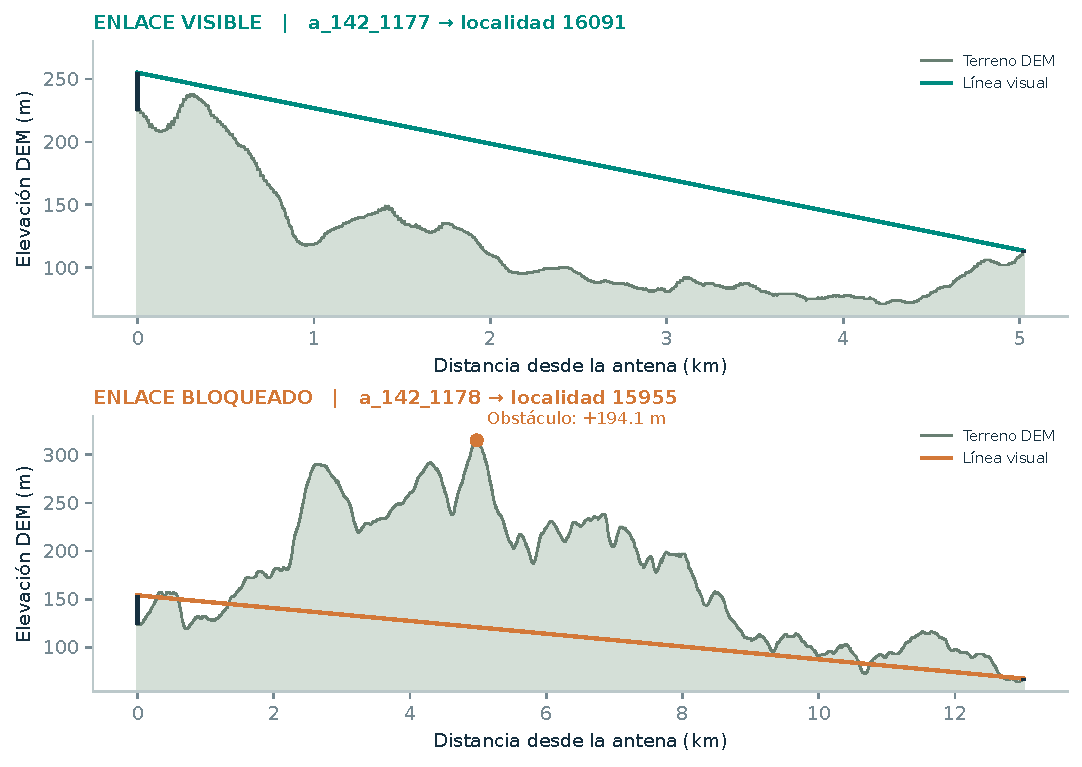
\includegraphics[width=.92\linewidth]{los_profiles.pdf}
\caption{Dos perfiles reales de elevación del piloto de Biobío.}
\label{fig:los}
\end{figure}

\clearpage
\section{Grafo de cobertura y solución óptima}

La matriz representa el grafo bipartito de Biobío. Las filas son candidatos, las columnas son localidades y una celda marcada indica que existe una arista de cobertura. Las filas iniciales corresponden a los cinco candidatos seleccionados por la enumeración exacta. El gráfico inferior muestra la población adicional asociada a esos candidatos en el orden estable de la solución devuelta.

\begin{figure}[h]
\centering
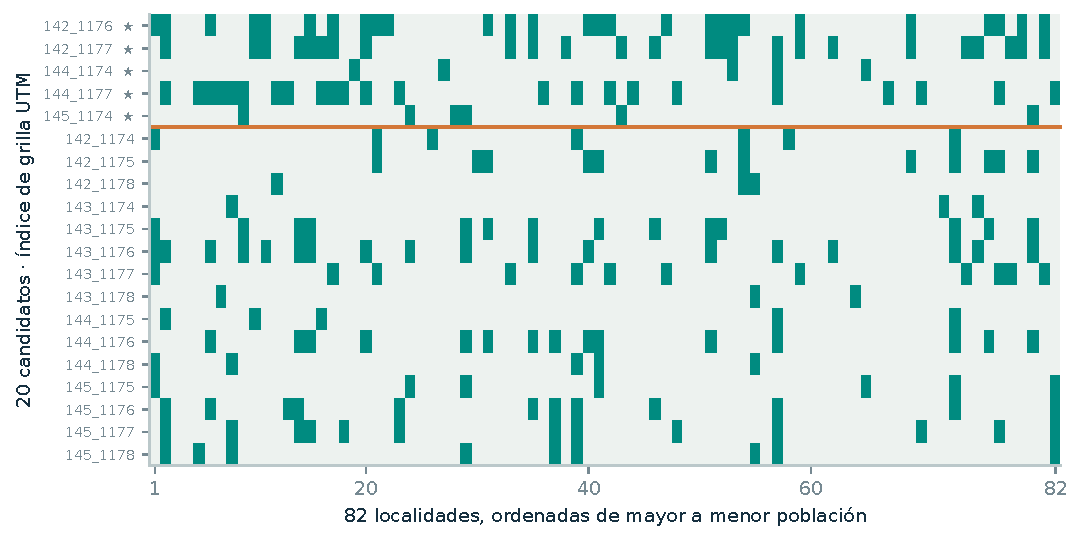
\includegraphics[width=\linewidth]{matrix.pdf}
\caption{Matriz de adyacencia del grafo bipartito del piloto de Biobío.}
\end{figure}

\begin{figure}[h]
\centering
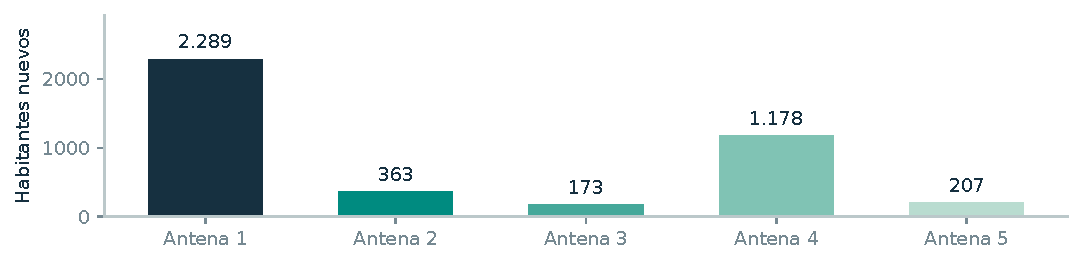
\includegraphics[width=\linewidth]{contributions.pdf}
\caption{Contribución de población única de los candidatos de la solución exacta de Biobío.}
\end{figure}

\clearpage
\section{Mapas de la solución exacta}

En los siguientes mapas, las estrellas muestran los candidatos elegidos por la enumeración exacta. Los puntos y límites de localidad permiten identificar la población cubierta bajo el modelo geométrico. Los mapas no representan infraestructura instalada ni cobertura comercial certificada.

\begin{figure}[h]
\centering
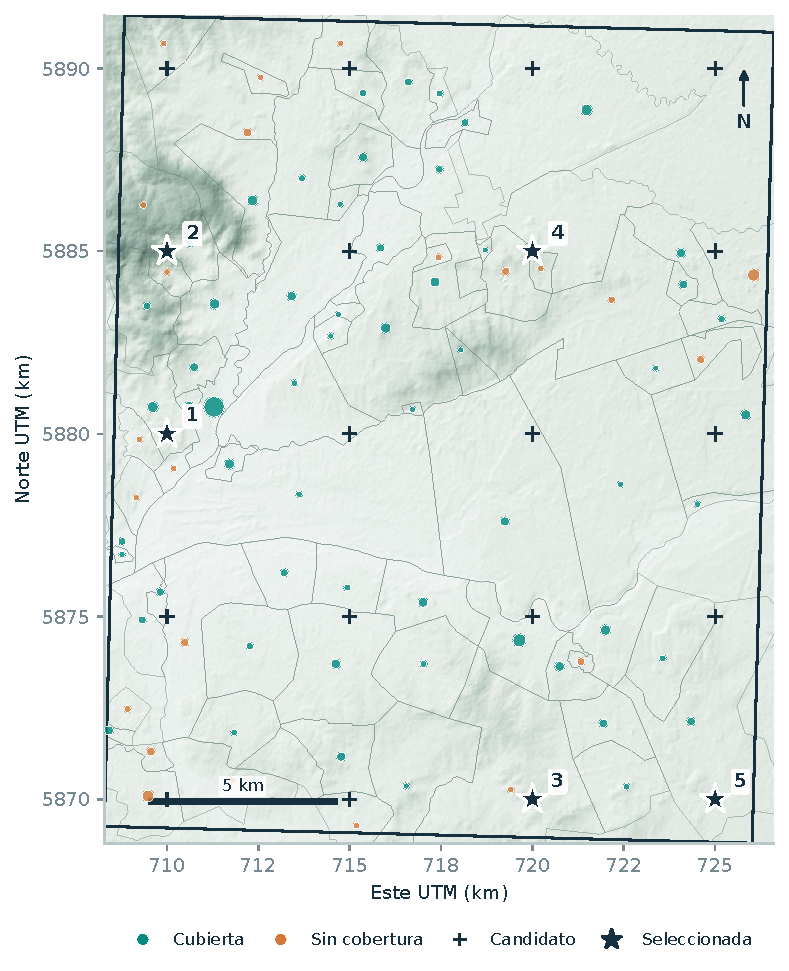
\includegraphics[width=.86\linewidth,height=.64\textheight,keepaspectratio]{map_biobio.pdf}
\caption{Piloto de Biobío: solución exacta con $k=5$.}
\end{figure}

\begin{figure}[h]
\centering
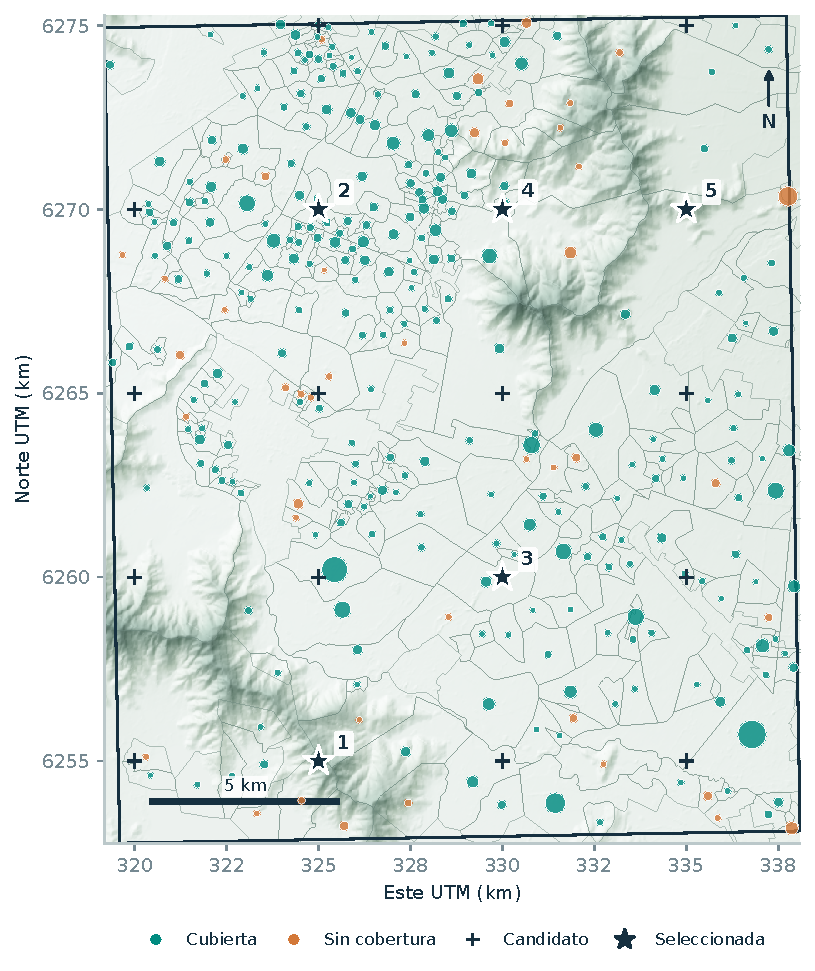
\includegraphics[width=.86\linewidth,height=.64\textheight,keepaspectratio]{map_metropolitana.pdf}
\caption{Piloto de Metropolitana: solución exacta con $k=5$.}
\end{figure}

\clearpage
\section{Cobertura alcanzada}

\begin{figure}[h]
\centering
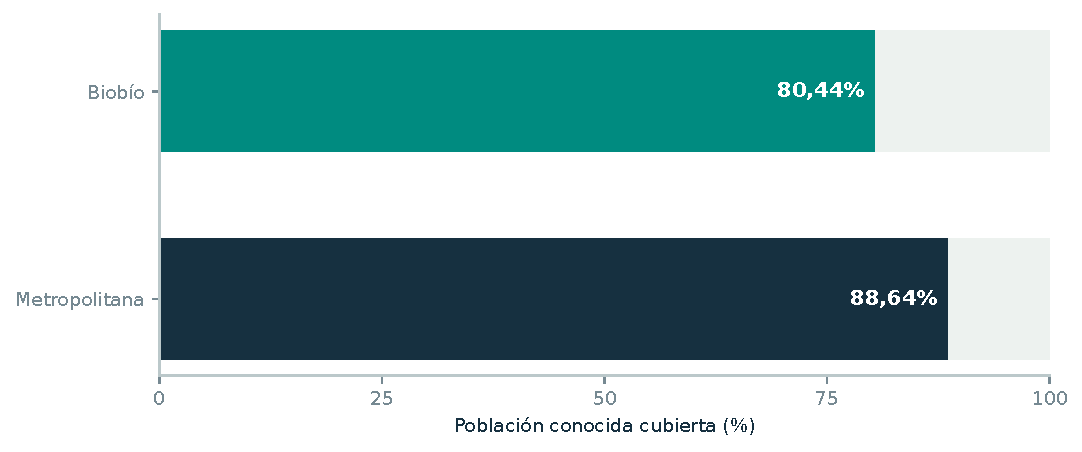
\includegraphics[width=.88\linewidth]{comparison.pdf}
\caption{Cobertura poblacional de la solución exacta en ambos pilotos.}
\end{figure}

\begin{center}
\begin{tabular}{@{}lrrr@{}}
\toprule
\textbf{Piloto} & \textbf{Localidades} & \textbf{Población cubierta} & \textbf{Cobertura} \\
\midrule
Biobío & 82 & 4.210 & 80,44\% \\
Metropolitana & 310 & 25.119 & 88,64\% \\
\bottomrule
\end{tabular}
\end{center}

La enumeración exacta revisa todas las combinaciones admisibles de hasta cinco candidatos, dentro del límite configurado de 100.000 combinaciones. En Biobío se evaluaron 15.504 combinaciones y en Metropolitana 11.628. Por ello, las dos selecciones mostradas son óptimas para sus respectivas instancias.

\end{document}
